
	\subsection{Пополнения}

	Пусть $A$~--- абелева группа с убывающей фильтрацией 
	\[
		A \supset A_0 \supset A_1 \supset \ldots A_n \supset
	\]

	$A$ можно сделать топологической группой, взяв в качестве базы окрестностей нуля $\{ A_n\}$. В нашем случае $A$ обычно будет кольцом или модулем, а фильтрация будет степенями идеала. 

	Ясно, что если $0 \neq a \in \bigcap A_i$, то её отделить от остальных не получится. Соотвественно, можно просто декларировать, что топология, заданная этой фильтрацией Хаусдорфова тогда и только тогда, когда 
	\[
		\bigcap_{i} A_i = 0. 
	\]

	Также заметим, что в этой топологии каждая $A_i$ будет не только открытой, но и замкнутой, так как все их сдвиги $x + A_i$ открыты, значит все смежные классы открыты и достаточно перейти к дополнению всех, кроме одного, откуда мы получим, что этот один смежный класс $y + A_j$ замкнут, следовательно $A_j$ замкнуто.

	Возьмём теперь пополнение по этой топологии. А именно, возьмём  прямой предел по следуюдщей последовательности: 
	\[
		\ldots \xrightarrow{\theta_2} A/A_2 \xrightarrow{\theta_1} A/A_1 \xrightarrow{\theta_0} A/A_0, \quad \widehat{A} \eqdef  \varprojlim A/A_{n}.
	\]

	\begin{definition} 
		Соотвественно, \emph{пополнением} $A$ в топологии, связанной с фильтрацией $\{ A_n \}$ называется определённое выше $\widehat{A}$.
	\end{definition}

	\begin{example}
		Например, $\Z_p = \varprojlim \Z/p^k\Z$ или $F[[t]] = \varprojlim F[t]/(t)^n$. 
	\end{example}

	Говорят, что фильтрации $(A_n)$ и $(B_n)$ имеют ограниченую разность, если 
	\[
		\exists n_0 \in \N \colon A_{n + n_0} \subset B_n \text{ и } B_{n + n_0} \subset A_n \ \forall \N.
	\]

	Ясно, что такие фильтрации задают одну и ту же топологию, но, на самом деле это условие сильнее (это мы поймём чуть попозже). 

	Напомним лемму о змее: 

	\begin{center}
		\textcolor{red}{сюда диаграмму про лемму о змее}
	\end{center}

	\begin{lemma} 
		Рассмотрим точную последовательность 
		\[
			0 \to A' \to A \to A'' \xrightarrow{p} 0, 
		\]
		$(A_n)$~--- фильтрация на $A$, $((A_n) \cap A')$~--- фильтрация на $A'$ и $(p(A_n))$ на A''. Тогда после перехода к пополнениям мы также получим точную последовательность 
		\[
			0 \to \widehat{A'} \to \widehat{A} \to \widehat{A''} \to 0.
		\]
	\end{lemma}
	\begin{proof}[Рабоче крестьянское доказательство] 
		Перейдём к точной последовательности: 
		\[
			0 \to A'/A_n \cap A' \to A/A_n \to A''/p(A_n)
		\]
		Определим теперь $\widetilde{A}$ и гомоморфизм $d$, как
		\[ 
			\widetilde{A} = \prod_{n = 0}^{\infty} A/A_n \xrightarrow{d} \widetilde{A}, \quad d((c_n)) = (c_n - \theta(c_{n + 1})). 
		\]

		Несложно заметить, что $\Ker{d} = \widehat{A}$. Соотвественно, надо рассмотреть диаграмму 
		\begin{center}
			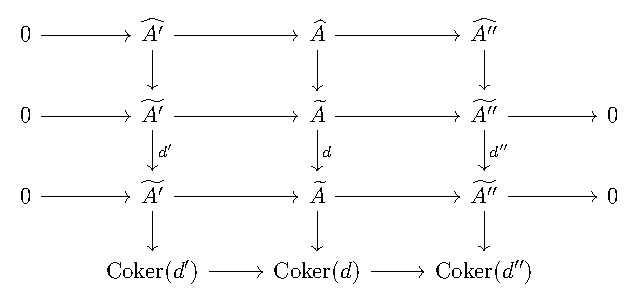
\includegraphics{lectures/3/commutative diagramms/snake_2.pdf}
		\end{center}

		и применить лемму о змее. Засчет сюръективности $\theta'$ $\ \forall (b_n)$ мы сможем подобрать $(c_n)$ такие, что $d'(c_n) = (b_n)$. А если $d'$ сюръективен, то $\Coker{d'} = 0$ и из леммы о змее мы получаем нужную  диаграмму:
		\[
			0 \to \widehat{A'} \to \widehat{A} \to \widehat{A''} \to \Coker{d'} = 0.
		\]

	\end{proof}
	\begin{proof}[Умновое доказательство]
		Оказывается, если существуют пределы $\lim{X_n}, \lim{Y_n}, \lim{Z_n}$ (где речь идет об объектах абелевой категории), то последовательность 
		\[
			0 \to \lim{X_n} \to \lim{Y_n} \to \lim{Z_n} 
		\]
		точна вообще всегегда, так как ядро~--- это предел, а пределы коммутируют, так как предельный функтор сопряжен к диагональному, а значит, сохраняет пределы. 
	\end{proof}

	\begin{corollary}
		$\widehat{A}/\widehat{A_n} \cong A/A_n$.
	\end{corollary}
	\begin{proof}
		Из прошлой леммы, полагая $A' = A_n$, мы получаем короткую точную последовательность 
		\[
			0 \to \widehat{A_n} \to \widehat{A} \to \widehat{A/A_n} \to 0
		\]

		А теперь заметим, что 
		\[
			(A/A_n) \supset A_1 / A_n \supset \ldots \supset A_n/A_n \supset 0 \supset \ldots, 
		\]
		откуда $\widehat{A/A_n} = A/A_n$ и из точности последоватльности выше мы получаем нужное. 
	\end{proof}

	\begin{corollary}
		Переходя в предыдущем следствии к пределу, мы получаем, что 
		\[
			\widehat{\widehat{A}} = \varprojlim \widehat{A}/\widehat{A_n} \cong \widehat{A},
		\]
		то есть пополение полно\footnote{что вполне логично. }
	\end{corollary}

	\begin{example}
		На простых примерах видна некоторая эвристика: $\Z \hookrightarrow \Z_{p}, \ F[t] \hookrightarrow F[[t]]$.
	\end{example}

	На самом деле, верно такое общее утверждение 
	
	\begin{theorem} 
		$\Ker\lr*{A \to \widehat{A}} = \bigcap_{n = 0}^{\infty} A_n$. 
	\end{theorem}

	\subsection{Градуированные алгебры и модули}

	\begin{definition} 
		Пусть $R_i$~--- $A$-модули. $R$ называют \emph{$\N$-градуированной $A$-алгеброй}, если 
		\[
			R = \bigoplus_{i = 0}^{\infty} R_i, \quad R_i \cdot R_j \subset  R_{i + j}.		
	 	\] 	

	 	\emph{Градуированным} $R$-модулем называют $M = \bigoplus M_i$ c условием $R_i M_j \subset M_{i + j}$.
	\end{definition}

	\begin{statement} 
		Градуированное кольцо $R$ является Нётеровым тогда и только тогда, когда $R_0$~--- нётерово и $R$~--- конечнопорожденная $R_0$-алгебра. 
	\end{statement}

	\begin{proof}
		В обратную сторону это почти очевидно: достаточно применить теорему Гильберта о Базисе и то, что нётеровость сохраняется при эпиморфизме. 

		Теперь докажем в обратную сторону.  Положим 
		\[
			R_{+} = \bigoplus_{n = 1}^{\infty} R_n \lei R,
		\]
		пусть $R_+$ порождён $\{ x_1, \ldots, x_s \}$  над $R$. Эти $x_i$ можно считать однородными, т.к. иначе разобьем на однородные компоненты, которые всё еще будут порождать. Таким образом, $x_i \in R_{k_i}$ для некоторого $k_i$. Возмём $y \in R_n$, 
		\[
			y = \sum_{j = 1}^{m} x_j z_j, \quad z_j \in R_{n - k_j}.
		\]

		По индукционному предположению $z_j \in R_0[x_1, \ldots, x_s] \implies y \in R_{0}[x_1, \ldots, x_s]$.
	\end{proof}

	Пусть $I \lei R$, расммотрим \emph{алгебру раздутия}: 
	\[
		\Bl_{I}\lr*{R} = \bigoplus_{n = 1}^{\infty} I^{n}. 
	\]
	



